\pdfminorversion=4
\documentclass[aspectratio=169]{beamer}

\mode<presentation>
{
  \usetheme{default}
  \usecolortheme{default}
  \usefonttheme{default}
  \setbeamertemplate{navigation symbols}{}
  \setbeamertemplate{caption}[numbered]
  \setbeamertemplate{footline}[frame number]  % or "page number"
  \setbeamercolor{frametitle}{fg=white}
  \setbeamercolor{footline}{fg=black}
}

\usepackage[english]{babel}
\usepackage[utf8x]{inputenc}
\usepackage{tikz}
\usepackage{courier}
\usepackage{array}
\usepackage{bold-extra}
\usepackage{minted}
\usepackage[thicklines]{cancel}
\usepackage{fancyvrb}

\xdefinecolor{dianablue}{rgb}{0.18,0.24,0.31}
\xdefinecolor{darkblue}{rgb}{0.1,0.1,0.7}
\xdefinecolor{darkgreen}{rgb}{0,0.5,0}
\xdefinecolor{darkgrey}{rgb}{0.35,0.35,0.35}
\xdefinecolor{darkorange}{rgb}{0.8,0.5,0}
\xdefinecolor{darkred}{rgb}{0.7,0,0}
\definecolor{darkgreen}{rgb}{0,0.6,0}
\definecolor{mauve}{rgb}{0.58,0,0.82}

\title[2019-05-22-pattern-matching-irishep]{Pattern matching for particle physics}
\author{Jim Pivarski}
\institute{Princeton University -- IRIS-HEP}
\date{May 22, 2019}

\usetikzlibrary{shapes.callouts}

\begin{document}

\logo{\pgfputat{\pgfxy(0.11, 7.4)}{\pgfbox[right,base]{\tikz{\filldraw[fill=dianablue, draw=none] (0 cm, 0 cm) rectangle (50 cm, 1 cm);}\mbox{\hspace{-8 cm}
\includegraphics[height=1 cm]{princeton-logo-long.png}\hspace{0.1 cm}\raisebox{0.1 cm}{
\includegraphics[height=0.8 cm]{iris-hep-logo-long.png}}\hspace{0.1 cm}}}}}

\begin{frame}
  \titlepage
\end{frame}

\logo{\pgfputat{\pgfxy(0.11, 7.4)}{\pgfbox[right,base]{\tikz{\filldraw[fill=dianablue, draw=none] (0 cm, 0 cm) rectangle (50 cm, 1 cm);}\mbox{\hspace{-8 cm}
\includegraphics[height=1 cm]{princeton-logo.png}\hspace{0.1 cm}\raisebox{0.1 cm}{
\includegraphics[height=0.8 cm]{iris-hep-logo.png}}\hspace{0.1 cm}}}}}

% Uncomment these lines for an automatically generated outline.
%\begin{frame}{Outline}
%  \tableofcontents
%\end{frame}

% START START START START START START START START START START START START START

\begin{frame}{}
\large
\vspace{1.25 cm}
Quite a few groups have been thinking about physics event processing languages, explicitly or implicitly.

\vspace{0.25 cm}
\begin{itemize}
\item \textcolor{darkblue}{LHADA/ADL:} Sezen Sekmen, Harry Prosper, Philippe Gras
\item \textcolor{darkblue}{CutLang:} Gokhan Unel
\item \textcolor{darkblue}{IRIS-HEP Analysis Systems:} Gordon Watts, Mason Proffitt, Emma Torro
\item \textcolor{darkblue}{FAST-Carpenter (YAML):} Benjamin Krikler
\item \textcolor{darkblue}{NAIL:} Andrea Rizzi
\item \textcolor{darkblue}{RDataFrame:} Enrico Guiraud, Danilo Piparo, and the ROOT Team
\item \textcolor{darkblue}{AEACuS \& RHADAManTHUS:} Joel Walker (phenomenology)
\item \textcolor{darkblue}{Femtocode:} me, though not for several years\ldots
\end{itemize}

\vspace{0.25 cm}
\small \hfill see \textcolor{blue}{\href{https://indico.cern.ch/event/769263/timetable/}{Analysis Description Languages Workshop}} (May 6--8)
\end{frame}

\begin{frame}{}
\Large
\vspace{1.25 cm}
\begin{columns}
\column{0.87\linewidth}
\begin{center}
For a physics domain-specific language (DSL) to be useful, it has to solve \textcolor{darkblue}{physics problems} in a way that is clearly simpler than the general-purpose language.

\vspace{1 cm}
\uncover<2->{This is different from just being ``high-level,'' solving any problem with less baggage than a low-level language.}
\end{center}
\end{columns}
\end{frame}

\begin{frame}{What is difficult in physics analyses?}
\large
\vspace{0.5 cm}
\begin{itemize}\setlength{\itemsep}{0.35 cm}
\item<1-> Distributing work to remote processors. General enough for a whole industry. (Spark, Parsl, Dask, Condor, Slurm\ldots)
\item<1-> Interactive analysis, publication-quality plotting. Also very general. (Jupyter)
\item<1-> Workflow management: chaining analysis tasks. General. (CWL, Makefile)
\item<2-> Booking, filling, managing histograms. \textcolor{darkblue}{Physics specific!} (ROOT)
\item<2-> Complex, multi-component distribution fitting. \textcolor{darkblue}{Physics specific!} (RooFit)
\item<2-> Complex multi-histogram fitting. \textcolor{darkblue}{Physics specific!} (Combine, HistFactory)
\item<3-> Signal/control regions, systematic variations. \textcolor{darkblue}{Physics specific!} (slide 2)
\item<3-> Particle combinatorics: complex decay chains. \textcolor{darkblue}{Physics specific!} (???)
\end{itemize}
\end{frame}

\begin{frame}[fragile]{Particle combinatorics}
\large
\vspace{0.35 cm}
Even a simple Z-peak requires combinatorics: don't double-count the muons!

\normalsize
\begin{minted}{c++}
std::vector<Particle> Z;
for (int i = 0;  i < muons.size();  i++)
    for (int j = i + 1;  j < muons.size();  j++)  // not all j
        Z.push_back(muons[i] + muons[j]);
\end{minted}

\large
This is the reason we can't ``just use SQL/Numpy/MATLAB.''

\vspace{0.25 cm}
\begin{uncoverenv}<2->
Awkward-Array addresses this with methods to generate per-event combinations.
\begin{itemize}
\item \mintinline{python}{A.cross(B)}: cross-join (Cartesian product) of \mintinline{python}{A} and \mintinline{python}{B}.
\item \mintinline{python}{A.pairs()}: inner-join of \mintinline{python}{A} with itself, excluding duplicates.
\item \mintinline{python}{A.distincts()}: inner-join of \mintinline{python}{A} with itself, also excluding $(A_i\mbox{, }A_i)$.
\item \mintinline{python}{A.choose(n)}: like \mintinline{python}{distincts}, but for tuples of size $n \le 5$.
\end{itemize}

\vspace{0.25 cm}
\textcolor{gray}{\normalsize (Cleverly implemented by Jaydeep Nandi and Nick Smith without internal for loops!)}
\vspace{0.1 cm}
\end{uncoverenv}
\end{frame}

\begin{frame}{But it's still not enough}
\Large
\vspace{0.25 cm}
\begin{center}
Building a complex decay chain using only these \\ combinatorial primitives would be a struggle.

\vspace{0.5 cm}
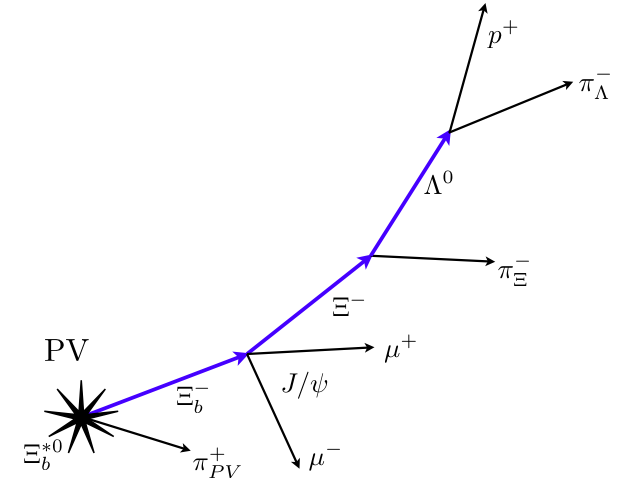
\includegraphics[width=0.5\linewidth]{decay-chain.png}
\end{center}
\end{frame}

\begin{frame}{Pattern matching}
\Large
\vspace{0.35 cm}
We want to fit a disconnected set of particles to a structured decay chain, which reminds me of pattern matching.

\vspace{0.5 cm}
\large
\begin{uncoverenv}<2->
Pattern matching is an uncommon programming language feature, like regular expressions, but for data structures: you make a model of what you want.

\vspace{0.25 cm}
\begin{center}
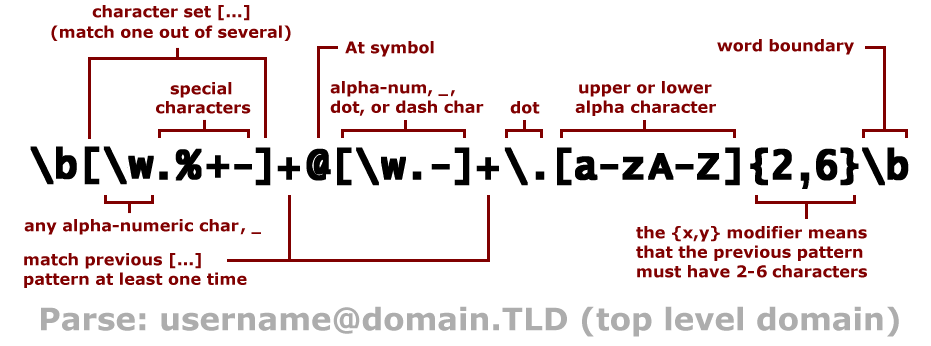
\includegraphics[width=0.8\linewidth]{regex-example.png}
\end{center}
\end{uncoverenv}
\end{frame}

\begin{frame}[fragile]{Examples of pattern matching}
\Large
\vspace{0.25 cm}
\textcolor{darkorange}{\bf Python:} \textcolor{gray}{(limited; can only unpack iterables)}

\begin{center}
\begin{minipage}{0.85\linewidth}
\normalsize
\begin{minted}{python}
def tree():
    return [[[1, 2], [3, 4]], [5, 6]]
(((a, b), c), _) = tree()    # a → 1, b → 2, c → [3, 4]
\end{minted}
\end{minipage}
\end{center}

\vspace{0.35 cm}
\begin{uncoverenv}<2->
\textcolor{darkorange}{\bf Haskell:}

\begin{center}
\begin{minipage}{0.85\linewidth}
\normalsize
\begin{minted}{haskell}
pz :: (Particle particle) => particle -> Float
pz (Neutral pt eta _)   = pt * sinh(eta)
pz (Charged pt eta _ q) = pt * sinh(eta)
\end{minted}
\end{minipage}
\end{center}
\end{uncoverenv}

\vspace{0.35 cm}
\begin{uncoverenv}<3->
\textcolor{darkorange}{\bf Scala:}

\begin{center}
\begin{minipage}{0.85\linewidth}
\normalsize
\begin{minted}{scala}
def pz(particle: Particle) = match particle {
    case Neutral(pt, eta, _)    => pt * sinh(eta)
    case Charged(pt, eta, _, q) => pt * sinh(eta)
}
\end{minted}
\end{minipage}
\end{center}
\end{uncoverenv}
\end{frame}

\begin{frame}[fragile]{Toy language with particle pattern matching}
\vspace{0.25 cm}
\scriptsize
\begin{Verbatim}[commandchars=\\\{\}]
start:      (NEWLINE | ";")* (statement (NEWLINE | ";")+)* statement (NEWLINE | ";")*

statement:  assignment | funcassign
funcassign: CNAME "(" [CNAME ("," CNAME)*] ")" "=" block
assignment: CNAME "=" expression

patassign:  CNAME "=" expression
          | CNAME "~" expression   -> symmetric
          | CNAME "~~" expression  -> all_symmetric
          | CNAME "!~" expression  -> asymmetric
          | CNAME "!~~" expression -> all_asymmetric
pattern:    (NEWLINE | ";")* (patassign (NEWLINE | ";")+)* patassign (NEWLINE | ";")*
function:   paramlist "=>" block

      \textcolor{darkblue}{... skip the boring part (standard expression grammar, same as Python) ...}

atom:       CNAME -> symbol | INT -> int | FLOAT -> float
          | "(" block ")" -> pass
          | "{" pattern "}" -> pass
          | "join" "{" pattern "}" -> join
\end{Verbatim}

\vspace{0.25 cm}
\fbox{{\normalsize\mbox{See }}\textcolor{blue}{\url{https://github.com/diana-hep/rejig/blob/master/pattern-match/define-and-run.py}}}
\end{frame}

\begin{frame}[fragile]{Example: Higgs $\to$ ZZ $\to$ $4\ell$}
\small
\begin{onlyenv}<1>
\begin{minted}{swift}
higgs(flavor1, flavor2) =
    join {
        z1 ~ {
            lep1 ~ flavor1
            lep2 ~ flavor1
            mass = (lep1.p4 + lep2.p4).mass
        }
        z2 ~ {
            lep1 ~ flavor2
            lep2 ~ flavor2
            mass = (lep1.p4 + lep2.p4).mass
        }
    }.filter(h => h.z1.lep1.charge != h.z1.lep2.charge and
                  h.z2.lep1.charge != h.z2.lep2.charge)
     .sort(h => (h.z1.mass - 91)**2 + (h.z2.mass - 91)**2)
\end{minted}
\begin{minted}{swift}
higgs4e    = higgs(electrons, electrons)
higgs4mu   = higgs(muons, muons)
higgs2e2mu = higgs(electrons, muons)
\end{minted}
\end{onlyenv}
\begin{onlyenv}<2>
\begin{minted}{swift}
higgs(flavor1, flavor2) =       // define a join pattern in a function
    join {
        z1 ~ {                  // Z boson subpattern
            lep1 ~ flavor1      // lep1, lep2 from flavor1 collection
            lep2 ~ flavor1      // leptons are NOT double-counted
            mass = (lep1.p4 + lep2.p4).mass
        }
        z2 ~ {                  // another Z boson
            lep1 ~ flavor2      // lep1, lep2 from flavor2, which
            lep2 ~ flavor2      // might be the same as flavor1
            mass = (lep1.p4 + lep2.p4).mass
        }                       // filter and sort with functionals
    }.filter(h => h.z1.lep1.charge != h.z1.lep2.charge and
                  h.z2.lep1.charge != h.z2.lep2.charge)
     .sort(h => (h.z1.mass - 91)**2 + (h.z2.mass - 91)**2)
\end{minted}
\begin{minted}{swift}
higgs4e    = higgs(electrons, electrons)    // use the function
higgs4mu   = higgs(muons, muons)            // to match patterns
higgs2e2mu = higgs(electrons, muons)
\end{minted}
\end{onlyenv}
\end{frame}

\begin{frame}[fragile]{Simpler, more pedagogical cases}
\vspace{0.25 cm}
\textcolor{darkblue}{\large\bf Input:}

\begin{minted}{swift}
x = [1.1, 2.2, 3.3, 4.4, 5.5]
y = ["one", "two", "three"]
\end{minted}

\vspace{0.25 cm}
\textcolor{darkblue}{\large\bf Expression:}

\begin{minted}{swift}
join {    // cross-join of the two (distinct) input collections
  a ~ x
  b ~ y
}
\end{minted}

\vspace{0.25 cm}
\textcolor{darkblue}{\large\bf Output:}

\begin{minted}[stripnl=false]{swift}
[(1.1, "one"),   (2.2, "one"),   (3.3, "one"),   (4.4, "one"),   (5.5, "one"),
 (1.1, "two"),   (2.2, "two"),   (3.3, "two"),   (4.4, "two"),   (5.5, "two"),
 (1.1, "three"), (2.2, "three"), (3.3, "three"), (4.4, "three"), (5.5, "three")]


\end{minted}
\end{frame}

\begin{frame}[fragile]{Simpler, more pedagogical cases}
\vspace{0.25 cm}
\textcolor{darkblue}{\large\bf Input:}

\begin{minted}{swift}
x = [1.1, 2.2, 3.3, 4.4, 5.5]
y = ["one", "two", "three"]
\end{minted}

\vspace{0.25 cm}
\textcolor{darkblue}{\large\bf Expression:}

\begin{minted}{swift}
join {    // inner join of one collection requiring uniqueness
  a ~ x
  b ~ x
}
\end{minted}

\vspace{0.25 cm}
\textcolor{darkblue}{\large\bf Output:}

\begin{minted}[stripnl=false]{swift}
[            (1.1, 2.2), (1.1, 3.3), (1.1, 4.4), (1.1, 5.5),
                         (2.2, 3.3), (2.2, 4.4), (2.2, 5.5),
                                     (3.3, 4.4), (3.3, 5.5),
                                                 (4.4, 5.5)]

\end{minted}
\end{frame}

\begin{frame}[fragile]{Simpler, more pedagogical cases}
\vspace{0.25 cm}
\textcolor{darkblue}{\large\bf Input:}

\begin{minted}{swift}
x = [1.1, 2.2, 3.3, 4.4, 5.5]
y = ["one", "two", "three"]
\end{minted}

\vspace{0.25 cm}
\textcolor{darkblue}{\large\bf Expression:}

\begin{minted}{swift}
join {    // two tildes doesn't require uniqueness
  a ~~ x
  b ~~ x
}
\end{minted}

\vspace{0.25 cm}
\textcolor{darkblue}{\large\bf Output:}

\begin{minted}{swift}
[(1.1, 1.1), (1.1, 2.2), (1.1, 3.3), (1.1, 4.4), (1.1, 5.5),
             (2.2, 2.2), (2.2, 3.3), (2.2, 4.4), (2.2, 5.5),
                         (3.3, 3.3), (3.3, 4.4), (3.3, 5.5),
                                     (4.4, 4.4), (4.4, 5.5),
                                                 (5.5, 5.5)]
\end{minted}
\end{frame}

\begin{frame}[fragile]{Simpler, more pedagogical cases}
\vspace{0.25 cm}
\textcolor{darkblue}{\large\bf Input:}

\begin{minted}{swift}
x = [1.1, 2.2, 3.3, 4.4, 5.5]
y = ["one", "two", "three"]
\end{minted}

\vspace{0.25 cm}
\textcolor{darkblue}{\large\bf Expression:}

\begin{minted}{swift}
join {    // exclamation point means don't constrain symmetry
  a !~ x
  b !~ x
}
\end{minted}

\vspace{0.25 cm}
\textcolor{darkblue}{\large\bf Output:}
\begin{minted}{swift}
[            (1.1, 2.2), (1.1, 3.3), (1.1, 4.4), (1.1, 5.5),
 (2.2, 1.1),             (2.2, 3.3), (2.2, 4.4), (2.2, 5.5),
 (3.3, 1.1), (3.3, 2.2),             (3.3, 4.4), (3.3, 5.5),
 (4.4, 1.1), (4.4, 2.2), (4.4, 3.3),             (4.4, 5.5),
 (5.5, 1.1), (5.5, 2.2), (5.5, 3.3), (5.5, 4.4)            ]
\end{minted}
\end{frame}

\begin{frame}[fragile]{Simpler, more pedagogical cases}
\vspace{0.25 cm}
\textcolor{darkblue}{\large\bf Input:}

\begin{minted}{swift}
x = [1.1, 2.2, 3.3, 4.4, 5.5]
y = ["one", "two", "three"]
\end{minted}

\vspace{0.25 cm}
\textcolor{darkblue}{\large\bf Expression:}

\begin{minted}{swift}
join {    // apply both operators for full generality
  a !~~ x
  b !~~ x
}
\end{minted}

\vspace{0.25 cm}
\textcolor{darkblue}{\large\bf Output:}
\begin{minted}{swift}
[(1.1, 1.1), (1.1, 2.2), (1.1, 3.3), (1.1, 4.4), (1.1, 5.5),
 (2.2, 1.1), (2.2, 2.2), (2.2, 3.3), (2.2, 4.4), (2.2, 5.5),
 (3.3, 1.1), (3.3, 2.2), (3.3, 3.3), (3.3, 4.4), (3.3, 5.5),
 (4.4, 1.1), (4.4, 2.2), (4.4, 3.3), (4.4, 4.4), (4.4, 5.5),
 (5.5, 1.1), (5.5, 2.2), (5.5, 3.3), (5.5, 4.4), (5.5, 5.5)]
\end{minted}
\end{frame}

\begin{frame}[fragile]{Simpler, more pedagogical cases}
\vspace{0.25 cm}
\textcolor{darkblue}{\large\bf Input:}

\begin{minted}{swift}
x = [1.1, 2.2, 3.3, 4.4, 5.5]
y = ["one", "two", "three"]
\end{minted}

\vspace{0.25 cm}
\textcolor{darkblue}{\large\bf Expression:}

\begin{minted}{swift}
join {    // separate nested structures break the symmetry
  a ~ x   // but uniqueness is global across the whole tree
  b ~ { c ~ x }
}
\end{minted}

\vspace{0.25 cm}
\textcolor{darkblue}{\large\bf Output:}

\begin{minted}[stripnl=false]{swift}
[            (1.1,(2.2)),(1.1,(3.3)),(1.1,(4.4)),(1.1,(5.5)),
 (2.2,(1.1)),            (2.2,(3.3)),(2.2,(4.4)),(2.2,(5.5)),
 (3.3,(1.1)),(3.3,(2.2)),            (3.3,(4.4)),(3.3,(5.5)),
 (4.4,(1.1)),(4.4,(2.2)),(4.4,(3.3)),            (4.4,(5.5)),
 (5.5,(1.1)),(5.5,(2.2)),(5.5,(3.3)),(5.5,(4.4))            ]
\end{minted}
\end{frame}

\begin{frame}[fragile]{Simpler, more pedagogical cases}
\vspace{0.25 cm}
\textcolor{darkblue}{\large\bf Input:}

\begin{minted}{swift}
x = [1.1, 2.2, 3.3, 4.4, 5.5]
y = ["one", "two", "three"]
\end{minted}

\vspace{0.25 cm}
\textcolor{darkblue}{\large\bf Expression:}

\begin{minted}{swift}
join {    // computing new fields doesn't change combinatorics
  a ~ x
  b ~ x
  c = a * b
}
\end{minted}

\vspace{0.25 cm}
\textcolor{darkblue}{\large\bf Output:}

\begin{minted}[stripnl=false]{swift}
[(1.1,2.2,2.42), (1.1,3.3,3.63), (1.1,4.4,4.84), (1.1,5.5,6.05),
                 (2.2,3.3,7.26), (2.2,4.4,9.68), (2.2,5.5,12.1),
                                 (3.3,4.4,14.5), (3.3,5.5,18.2),
                                                 (4.4,5.5,24.2)]

\end{minted}
\end{frame}

\begin{frame}[fragile]{Simpler, more pedagogical cases}
\vspace{0.25 cm}
\textcolor{darkblue}{\large\bf Input:}

\begin{minted}{swift}
x = [1.1, 2.2, 3.3, 4.4, 5.5]
y = ["one", "two", "three"]
\end{minted}

\vspace{0.25 cm}
\textcolor{darkblue}{\large\bf Expression:}

\begin{minted}{swift}
join {    // not all fields need to be matches
  a ~ x
  b = y
}
\end{minted}

\vspace{0.25 cm}
\textcolor{darkblue}{\large\bf Output:}

\begin{minted}[stripnl=false]{swift}
[(1.1, ["one", "two", "three"]),
 (2.2, ["one", "two", "three"]),
 (3.3, ["one", "two", "three"]),
 (4.4, ["one", "two", "three"]),
 (5.5, ["one", "two", "three"])]
\end{minted}
\end{frame}

\begin{frame}[fragile]{Simpler, more pedagogical cases}
\vspace{0.25 cm}
\textcolor{darkblue}{\large\bf Input:}

\begin{minted}{swift}
x = [1.1, 2.2, 3.3, 4.4, 5.5]
y = ["one", "two", "three"]
\end{minted}

\vspace{0.25 cm}
\textcolor{darkblue}{\large\bf Expression:}

\begin{minted}{swift}
join {    // in fact, none of them really need to be
  a = x
  b = y
}
\end{minted}

\vspace{0.25 cm}
\textcolor{darkblue}{\large\bf Output:}

\begin{minted}[stripnl=false]{swift}
[([1.1, 2.2, 3.3, 4.4, 5.5], ["one", "two", "three"])]




\end{minted}
\end{frame}

\begin{frame}[fragile]{Simpler, more pedagogical cases}
\vspace{0.25 cm}
\textcolor{darkblue}{\large\bf Input:}

\begin{minted}{swift}
x = [1.1, 2.2, 3.3, 4.4, 5.5]
y = ["one", "two", "three"]
\end{minted}

\vspace{0.25 cm}
\textcolor{darkblue}{\large\bf Expression:}

\begin{minted}{swift}
join {    // joins can be nested, but the matches don't mix
  a = x
  b = join { c ~ x }        // a and c can match the same x
}
\end{minted}

\vspace{0.25 cm}
\textcolor{darkblue}{\large\bf Output:}

\begin{minted}[stripnl=false]{swift}
[(1.1, [1.1, 2.2, 3.3, 4.4, 5.5]),
 (2.2, [1.1, 2.2, 3.3, 4.4, 5.5]),
 (3.3, [1.1, 2.2, 3.3, 4.4, 5.5]),
 (4.4, [1.1, 2.2, 3.3, 4.4, 5.5]),
 (5.5, [1.1, 2.2, 3.3, 4.4, 5.5])]
\end{minted}
\end{frame}

\begin{frame}[fragile]{Back to example: Higgs $\to$ ZZ $\to$ $4\ell$}
\small
\begin{minted}{swift}
higgs(flavor1, flavor2) =
    join {
        z1 ~ {
            lep1 ~ flavor1
            lep2 ~ flavor1
            mass = (lep1.p4 + lep2.p4).mass
        }
        z2 ~ {
            lep1 ~ flavor2
            lep2 ~ flavor2
            mass = (lep1.p4 + lep2.p4).mass
        }
    }.filter(h => h.z1.lep1.charge != h.z1.lep2.charge and
                  h.z2.lep1.charge != h.z2.lep2.charge)
     .sort(h => (h.z1.mass - 91)**2 + (h.z2.mass - 91)**2)
\end{minted}
\begin{minted}{swift}
higgs4e    = higgs(electrons, electrons)
higgs4mu   = higgs(muons, muons)
higgs2e2mu = higgs(electrons, muons)
\end{minted}
\end{frame}

\begin{frame}[fragile]{A good formalism is usable in other contexts}
\small
\vspace{0.5 cm}
\textcolor{darkblue}{\large Example: gen-reco matching}

\vspace{-0.25 cm}
\begin{columns}
\column{0.9\linewidth}
\begin{minted}{swift}
matched_gens =
    join {
        // gen is a single element
        gen ~ gens
        // matched is a list with zero or one elements
        matched = recos.sort(x => delta_R(gen, x.reco))[:1]
    }.filter(x => len(x.matched) > 0)
\end{minted}
\end{columns}

\vspace{0.25 cm}
\textcolor{gray}{\normalsize (One matched collection, one reduced---makes asymmetry explicit.)}

\vspace{0.65 cm}
\textcolor{darkblue}{\large Example: jet cleaning}

\vspace{-0.25 cm}
\begin{columns}
\column{0.9\linewidth}
\begin{minted}{swift}
clean_jets =
    jets.filter(jet => leptons.map(
        lepton => delta_R(jet, lepton) < 0.5).any())
\end{minted}
\end{columns}

\vspace{0.25 cm}
\textcolor{gray}{\normalsize (Doesn't even need matched collections.)}
\end{frame}

\begin{frame}{What about syntax?}
\Large
\vspace{0.5 cm}
\textcolor{darkblue}{This was an example syntax in a toy language:} in no way final.

\large
\vspace{0.5 cm}
\begin{itemize}\setlength{\itemsep}{0.5 cm}
\item Grammar requires an Earley algorithm (slow); may want to finagle it to work with LALR (fast).
\item It might be possible to embed this in a host language like C++ or Python, but at the expense of readability (in my attempts).
\item What about two-dimensional syntax? (Next page.)
\end{itemize}
\end{frame}

\begin{frame}[fragile]{Behold Racket (Scheme)'s two-dimensional syntax}
\normalsize
\vspace{0.5 cm}

\begin{center}
\begin{minipage}{0.8\linewidth}
\begin{minted}{scheme}
(define (subtype? a b)
  #2dmatch
  +----------+----------+-------+----------+
  |   a  b   | 'Integer | 'Real | 'Complex |
  +----------+----------+-------+----------+
  | 'Integer |             #t              |
  +----------+----------+                  |
  | 'Real    |          |                  |
  +----------+          +-------+          |
  | 'Complex |        #f        |          |
  +----------+------------------+----------+)
\end{minted}
\end{minipage}
\end{center}

\vspace{0.25 cm}
\small \hfill See \textcolor{blue}{\url{https://docs.racket-lang.org/2d/index.html}}
\end{frame}

\begin{frame}[fragile]{So maybe something like this?}
\large
\vspace{0.25 cm}
The ASCII art of the decay would literally be the code used to match it.

\normalsize
\vspace{0.5 cm}
\begin{Verbatim}[commandchars=\\\{\}]
Higgs: sort (Z1.mass - 91)**2 + (Z2.mass - 91)**2
   |
   +--> Z1: cut lep1.charge != lep2.charge
   |     +--> lep1, lep2 in electrons or lep1, lep2 in muons
   |
   +--> Z2: cut lep3.charge != lep4.charge
         +--> lep3, lep4 in electrons or lep3, lep4 in muons
\end{Verbatim}

\large
\vspace{0.5 cm}
Maybe the arrows are unnecessary; maybe an indentation rule like Python's?
\end{frame}

\begin{frame}{}
\Large
\vspace{1.25 cm}
\begin{center}
Maybe not.
\end{center}
\end{frame}

\begin{frame}{Conclusions}
\Large
\vspace{0.5 cm}
\begin{itemize}
\item Investigated the use of a pattern-matching syntax to match particle decay chains.
\end{itemize}
\end{frame}

\end{document}
